To aid in the computation of the examples presented in this thesis, we use a tool called \relview. \relview\index{\relview}\ is an interactive tool for computer-aided manipulation of relations represented as Boolean matrices. It is developed at the Department of Computer Science and Applied Mathematics at Christian-Albrechts-University in Kiel, Germany~\cite{relview}. This appendix presents an overview of working with \relview\ and the programs developed in \relview\ to automate the tests and computations of the corollaries presented in Chapter~\ref{cha:formulation_of_a_detection_technique}.

\section{Working With \relview}
\label{sec:working_with_relview}
% Begin Section

In this section, we look at how to work with relations using the \relview\ tool. The information presented in this section is taken from~\cite{Behnke2009aa}.

\subsection{Representing Relations}
\label{sub:representing_relations}
% Begin SubSection

\relview\ is able to represent relations both as Boolean matrices and as an ASCII description.

\subsubsection{Boolean Matrix Representation}
\label{ssub:boolean_matrix_representation}
% Begin SubSubSection

The Boolean matrix representation\index{relation!Boolean matrix representation} of relations in \relview\ is a graphical representation. A relation is given as a matrix where the rows represent the domain of the relation and the columns represent the range of the relation. A filled in cell of the matrix represents that element being included in the relation. An example of Boolean matrix representation of a relation in \relview\ is given in Figure~\ref{fig:matrix_example}. \newline

\begin{figure}[ht]
	\centering
	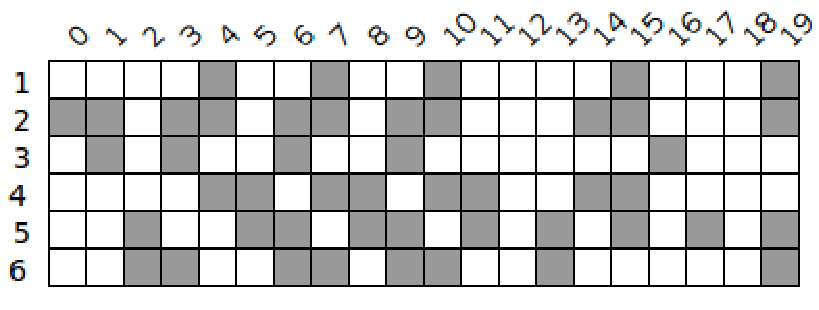
\includegraphics[scale=0.65]{Figures/PDF/Relview/NoiseQ.pdf}
	\caption{Example of the Boolean matrix representation of a relation in \relview.}
	\label{fig:matrix_example}
\end{figure}

% End SubSubSection

\subsubsection{ASCII Representation}
\label{ssub:ascii_representation}
% Begin SubSubSection

The ASCII representation\index{relation!ASCII representation} of relations in \relview\ is a textual representation. A relation is given as a list entries of the form ``\texttt{Domain : Range}''. The ASCII representation of the relation given in Figure~\ref{fig:matrix_example} is given below. \newpage

\begin{lstlisting}
	R (6, 20)
	1 : 5, 8, 11, 16, 20
	2 : 1, 2, 4, 5, 7, 8, 10, 11, 15, 16, 20
	3 : 2, 4, 7, 10, 17
	4 : 5, 6, 8, 9, 11, 12, 15, 16
	5 : 3, 6, 7, 9, 10, 12, 14, 16, 18, 20
	6 : 3, 4, 7, 8, 10, 11, 14, 20
\end{lstlisting}~

% End SubSubSection

% End SubSection

\subsection{Operations}
\label{sub:operations}
% Begin SubSection

\begin{table}[ht]
\label{tbl:bool_ops}
	\centering
	\begin{tabular}{|r|l|}
		\hline
		Syntax & Description \\ \hline \hline
		$-R$ &  Complement\index{complement} of relation $R$\\ 
		$R \;|\; S$ & Union\index{set!union} (join) of $R$ and $S$ \\ 
		$R \;\&\; S$ & Intersection\index{set!intersection} (meet) of $R$ and $S$ \\  
		$R + S$ & Relational sum\index{relational sum} of $R$ and $S$ \\  \hline 
	\end{tabular}
	\caption{Boolean Operations}					
\end{table} ~

\begin{table}[ht]
\label{tbl:RA_ops}
	\centering
	\begin{tabular}{|r|l|}
		\hline
		Syntax & Description \\ \hline \hline
		$R\;\hat{}$ & Converse\index{converse} of relation $R$ \\ 
		$R \;*\; S$ & Composition\index{composition} of $R$ and $S$ \\ \hline 
	\end{tabular}
	\caption{Relational Algebraic Operations}					
\end{table} ~

\begin{table}[ht]
\label{tbl:residual_ops}
	\centering
	\begin{tabular}{|r|l|}
		\hline
		Syntax & Description \\ \hline \hline
		$\RAleftresidual{S}{R}$ & Left residue\index{residue!left residue} of $R$ and $S$ \\ 
		$\RArightresidual{R}{S}$ & Right residue\index{residue!right residue} of $R$ and $S$ \\  
		$syq(R,S)$ & Symmetric quotient\index{symmetric quotient} of $R$ and $S$ \\  \hline 
	\end{tabular}
	\caption{Residuals and Symmetric Quotients}					
\end{table} ~

\begin{table}[ht]
\label{tbl:test_ops}
	\centering
	\begin{tabular}{|r|l|}
		\hline
		Syntax & Description \\ \hline \hline
		$eq(R,S)$ &  Test, whether $R$ and $S$ are equal \\ 
		$incl(R,S)$ &  Test, whether $R$ is included in $S$ \\  \hline 
	\end{tabular}
	\caption{Relational Tests}					
\end{table}~

% End SubSection

\subsection{Labels}
\label{sub:labels}
% Begin SubSection

	Labels are organized into sets which are mappings from natural numbers to labels or identifiers. \newline
	
	The labels that are used in this thesis are given below: \newline
	
	\begin{lstlisting}
		Digit = { 1 "0", 2 "1", 3 "2", 4 "3", 5 "4", 6 "5", 7 "6", 8 "7", 9 "8", 10 "9" }
		
		Encryption = { 1 "0", 2 "1", 3 "2", 4 "3", 5 "4", 6 "5", 7 "6", 8 "7", 9 "8", 10 "9", 11 "10", 12 "11", 13 "12", 14 "13", 15 "14", 16 "15", 17 "16", 18 "17", 19 "18", 20 "19" }
		
		Bool = { 1 "True?" }
	\end{lstlisting}
	~
	
	These labels are used in the Boolean matrix representation of relations making them easier to read and understand. The label ``Digit'' corresponds to the digit data type, the label ``Encryption'' corresponds to the natural numbers which can be used to encrypt the digits, and the label ``Bool'' simply adds a descriptive label for boolean results. \newline
	
	It is important to note that when representing relations using labels, the ASCII representation of the relation must correspond to the natural number and not the label or identifier. For example, if we want to represent the digit 4 being sent at time 1, \ie $(1,4)$ we must use ``1 : 5'' in the ASCII representation so that the label corresponds to the digit 4.

% End SubSection

\subsection{Truth Values}
\label{sub:truth_values}
% Begin SubSection

	In \relview, the result of a Boolean operation is a $1 \times 1$ Boolean matrix with the truth values corresponding to $\RAtop = \true$ and $\RAbot = \false$. This is to say that the truth values are given by the Boolean matrices given in Figure~\ref{fig:truthvalues}. \newline

	\begin{figure}[ht]
		\centering
		\subfigure[True]{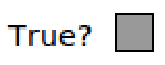
\includegraphics[scale=0.65]{Figures/PDF/Relview/True.pdf}} \hspace{1in}
		\subfigure[False]{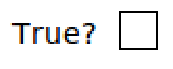
\includegraphics[scale=0.65]{Figures/PDF/Relview/False.pdf}}
		\caption{\relview\ representation of truth values.}
		\label{fig:truthvalues}
	\end{figure}

% End SubSection

% End Section

\section{\relview\ Programs}
\label{sec:relview_programs}
% Begin Section

Program~\ref{prog:test} represents the test outlined in Corollary~\ref{cor:test}. \newpage

\begin{program}
\label{prog:test}~
	\begin{lstlisting}
		Test(p,q)
		    DECL test1, test2, res
		    BEG  test1 = eq(p,q*(q\p));
		         test2 = eq(q,p*(p\q));
		         res = test1 | test2
		         RETURN res
		    END.
	\end{lstlisting}
\end{program}

Program~\ref{prog:compute} corresponds to the computations presented in Corollary~\ref{cor:compute}. 

\begin{program}
\label{prog:compute}~
	\begin{lstlisting}
		Compute(p, q, r)
		    DECL test1, test2, res
		    BEG  test1 = incl(p,q*(r^ & (q\p)));
		         test2 = incl(q,p*(r  & (p\q)));
		         IF test1 & test2
		            THEN res = r & syq(p,q)
		            ELSE IF test1
		               THEN res = r & (q\p)^
		               ELSE IF test2
		                  THEN res = r & (p\q)
		                  ELSE res = false 
		               FI 
		            FI 
		         FI       
		         RETURN res
		    END.
	\end{lstlisting}
\end{program}

\newpage
Program~\ref{prog:compute_bij} automates the computation given in Corollary~\ref{cor:compute_bij}. 

\begin{program}
\label{prog:compute_bij}~
	\begin{lstlisting}
		ComputeBij(p, q, r)
		    DECL test1, test2, res
		    BEG  IF eq((p\q),(q\p)^)
		            THEN res = r & (p\q)
		            ELSE res = false 
		         FI       
		         RETURN res
		    END.		
	\end{lstlisting}
\end{program}

% End Section